
\subsection{Answers}
\begin{table}[htb]%
\begin{center}%
\caption{Q3: In the tradeoff between code portability and performance, which is more or less important for you to write MPI programs? ["1" means portability is the most important and "3" means both are equally...}%
\label{tab:Q3-ans}%
\begin{tabular}{l|l|r}%
\hline%
Choice & Abbrv. & \# Answers \\%
\hline%
1 & Low & 1 (9.1\%) \\%
2 & 2 & 2 (18.2\%) \\%
3 & 3 & 4 (36.4\%) \\%
4 & 4 & 2 (18.2\%) \\%
5 & 5 & 2 (18.2\%) \\%
6 & High & 0 (0.0\%) \\%
\hline%
\multicolumn{2}{c}{total} & 11 \\%
\hline%
\end{tabular}%
\end{center}%
\end{table}%


People with high MPI skills who chose MPI skill 4 or higher 
account for 65\% of the respondents. This 
indicates that people with high MPI skills have shown 
interest in our research, and/or people with low MPI skill did not
find confident enough to answer this survey. It should be noted that
the most skillful MPI experts in USA occupy more than 20~\%. 

\begin{figure}[htb]
\begin{center}
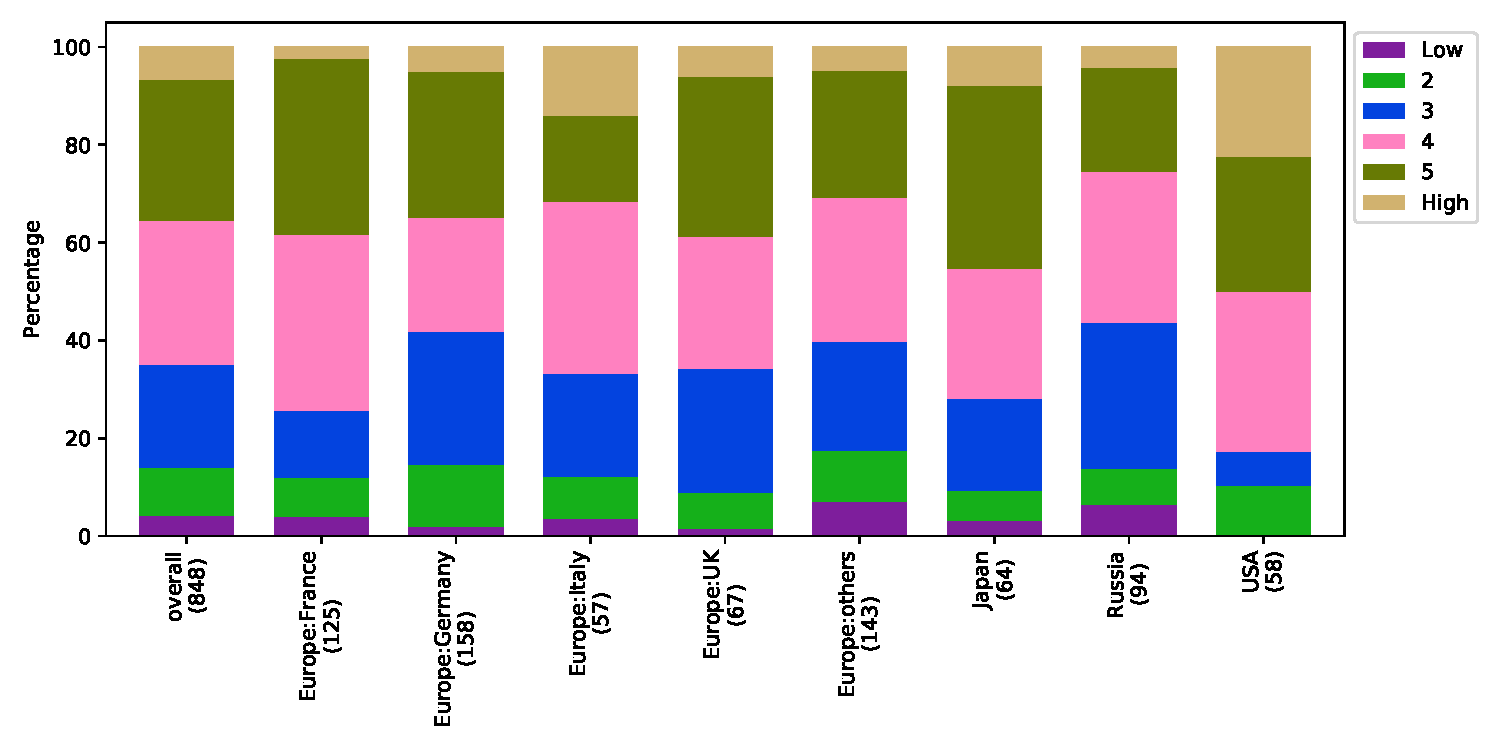
\includegraphics[width=10cm]{../pdfs/Q3.pdf}
\caption{Simple analysis: Q3}
\label{fig:Q3}
\end{center}
\end{figure}

Figure~\ref{fig:Q2-Q3X} shows the cross-tab between Q2 and Q3. If there
is high correlation between the programming skill and MPI skill, the
dark cells could be seen as a diagonal line from the top-left to
down-right. This line can be seen in Italy, Russia and USA. However,
the situations between Russia and USA look very different. In Russia,
the diagonal line can be seen near the center of the heatmap, whereas
the disagonal line of USA is off to the lower-right. This means the
many of MPI programmers in USA are more talented than the other
countries. 

\begin{figure}[htb]
\begin{center}
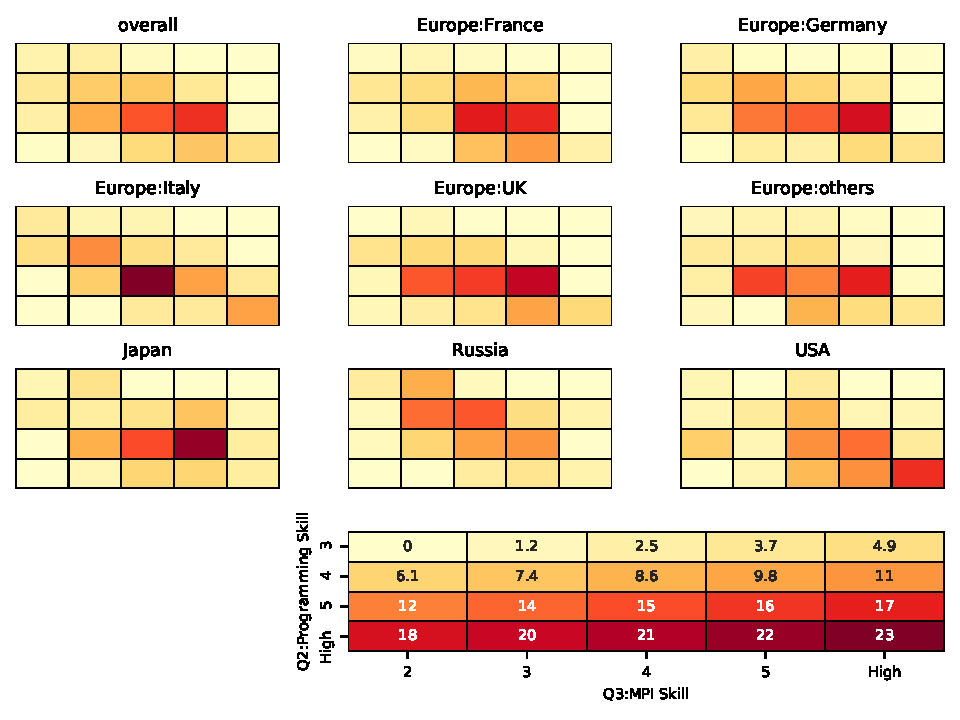
\includegraphics[width=10cm]{../pdfs/Q2-Q3.pdf}
\caption{Cross-tab analysis: Q2 and Q3}
\label{fig:Q2-Q3X}
\end{center}
\end{figure}
